% This document is the template for the talks given at the Matheon Center Days March 12-14, 2012..
%
%Please time your presentation for 10 minutes plus 5 minutes questioning.
%
% The beamerMatheon class was created for the
%
%          DFG Research Center Matheon
%          Mathematics for Key Technologies
%
% Please send corrections and suggestions to webmaster@matheon.de
%
% use the beamer class:
\documentclass[12pt]{beamer}

% use the beamerMatheon theme with english titles
\mode<presentation>{\usetheme[language=english]{Matheon}}
\setbeamertemplate{navigation symbols}{}%remove navigation symbols
\setbeamercovered{transparent=50}

% used packages
\usepackage[T1]{fontenc}
\usepackage{amsmath}
\usepackage{amssymb}
\usepackage{alltt}
\usepackage{url}
\usepackage{graphicx}\graphicspath{{../images/}{../figures/}{./image/}}
\usepackage{multirow}
\usepackage{color}
\usepackage{contour}
\contournumber{32}
\contourlength{0.1em}

\newcommand*{\vcenteredhbox}[1]{\begingroup
\setbox0=\hbox{#1}\parbox{\wd0}{\box0}\endgroup}



% ----------- title ------------------------------------------

\title{\vspace{-1cm}Quasiisothermic Mesh Layout}

\author{Stefan~Sechelmann}
\institute{Institut f\"ur Mathematik, TU-Berlin}
\jointwork{joint work with\\
Thilo~R\"orig and Alexander~I.~Bobenko
}

\date{}

\pgfdeclareimage[height=1.2cm]{logo}{logotext.pdf}
%\insertLogo{logo}
% insert logo of instute if wanted     *** use one of the following commands instead of the two lines above

%\insertLogoZIB
%\insertLogoFU
%\insertLogoHU
\insertLogoTU
%\insertLogoWIAS
%\insertLogoZIB

% set information on every page
\footinformation{Stefan Sechelmann - Quasiisothermic Mesh Layout}


% ----------- document ------------------------------------------
\begin{document}

% set title
\maketitle

\section{Quasiisothermic Mesh Layout}

\begin{frame}
	\frametitle{Quasiisothermic Mesh Layout}
	\begin{center}
		\includegraphics[width=0.6\linewidth]{cover01_lupe.png}
	\\
		Triangulated Surface
	\end{center}
\end{frame}

\begin{frame}
	\frametitle{Quasiisothermic Mesh Layout}
	\begin{center}
		\includegraphics[width=0.48\linewidth]{cover03_no_directions.png}
		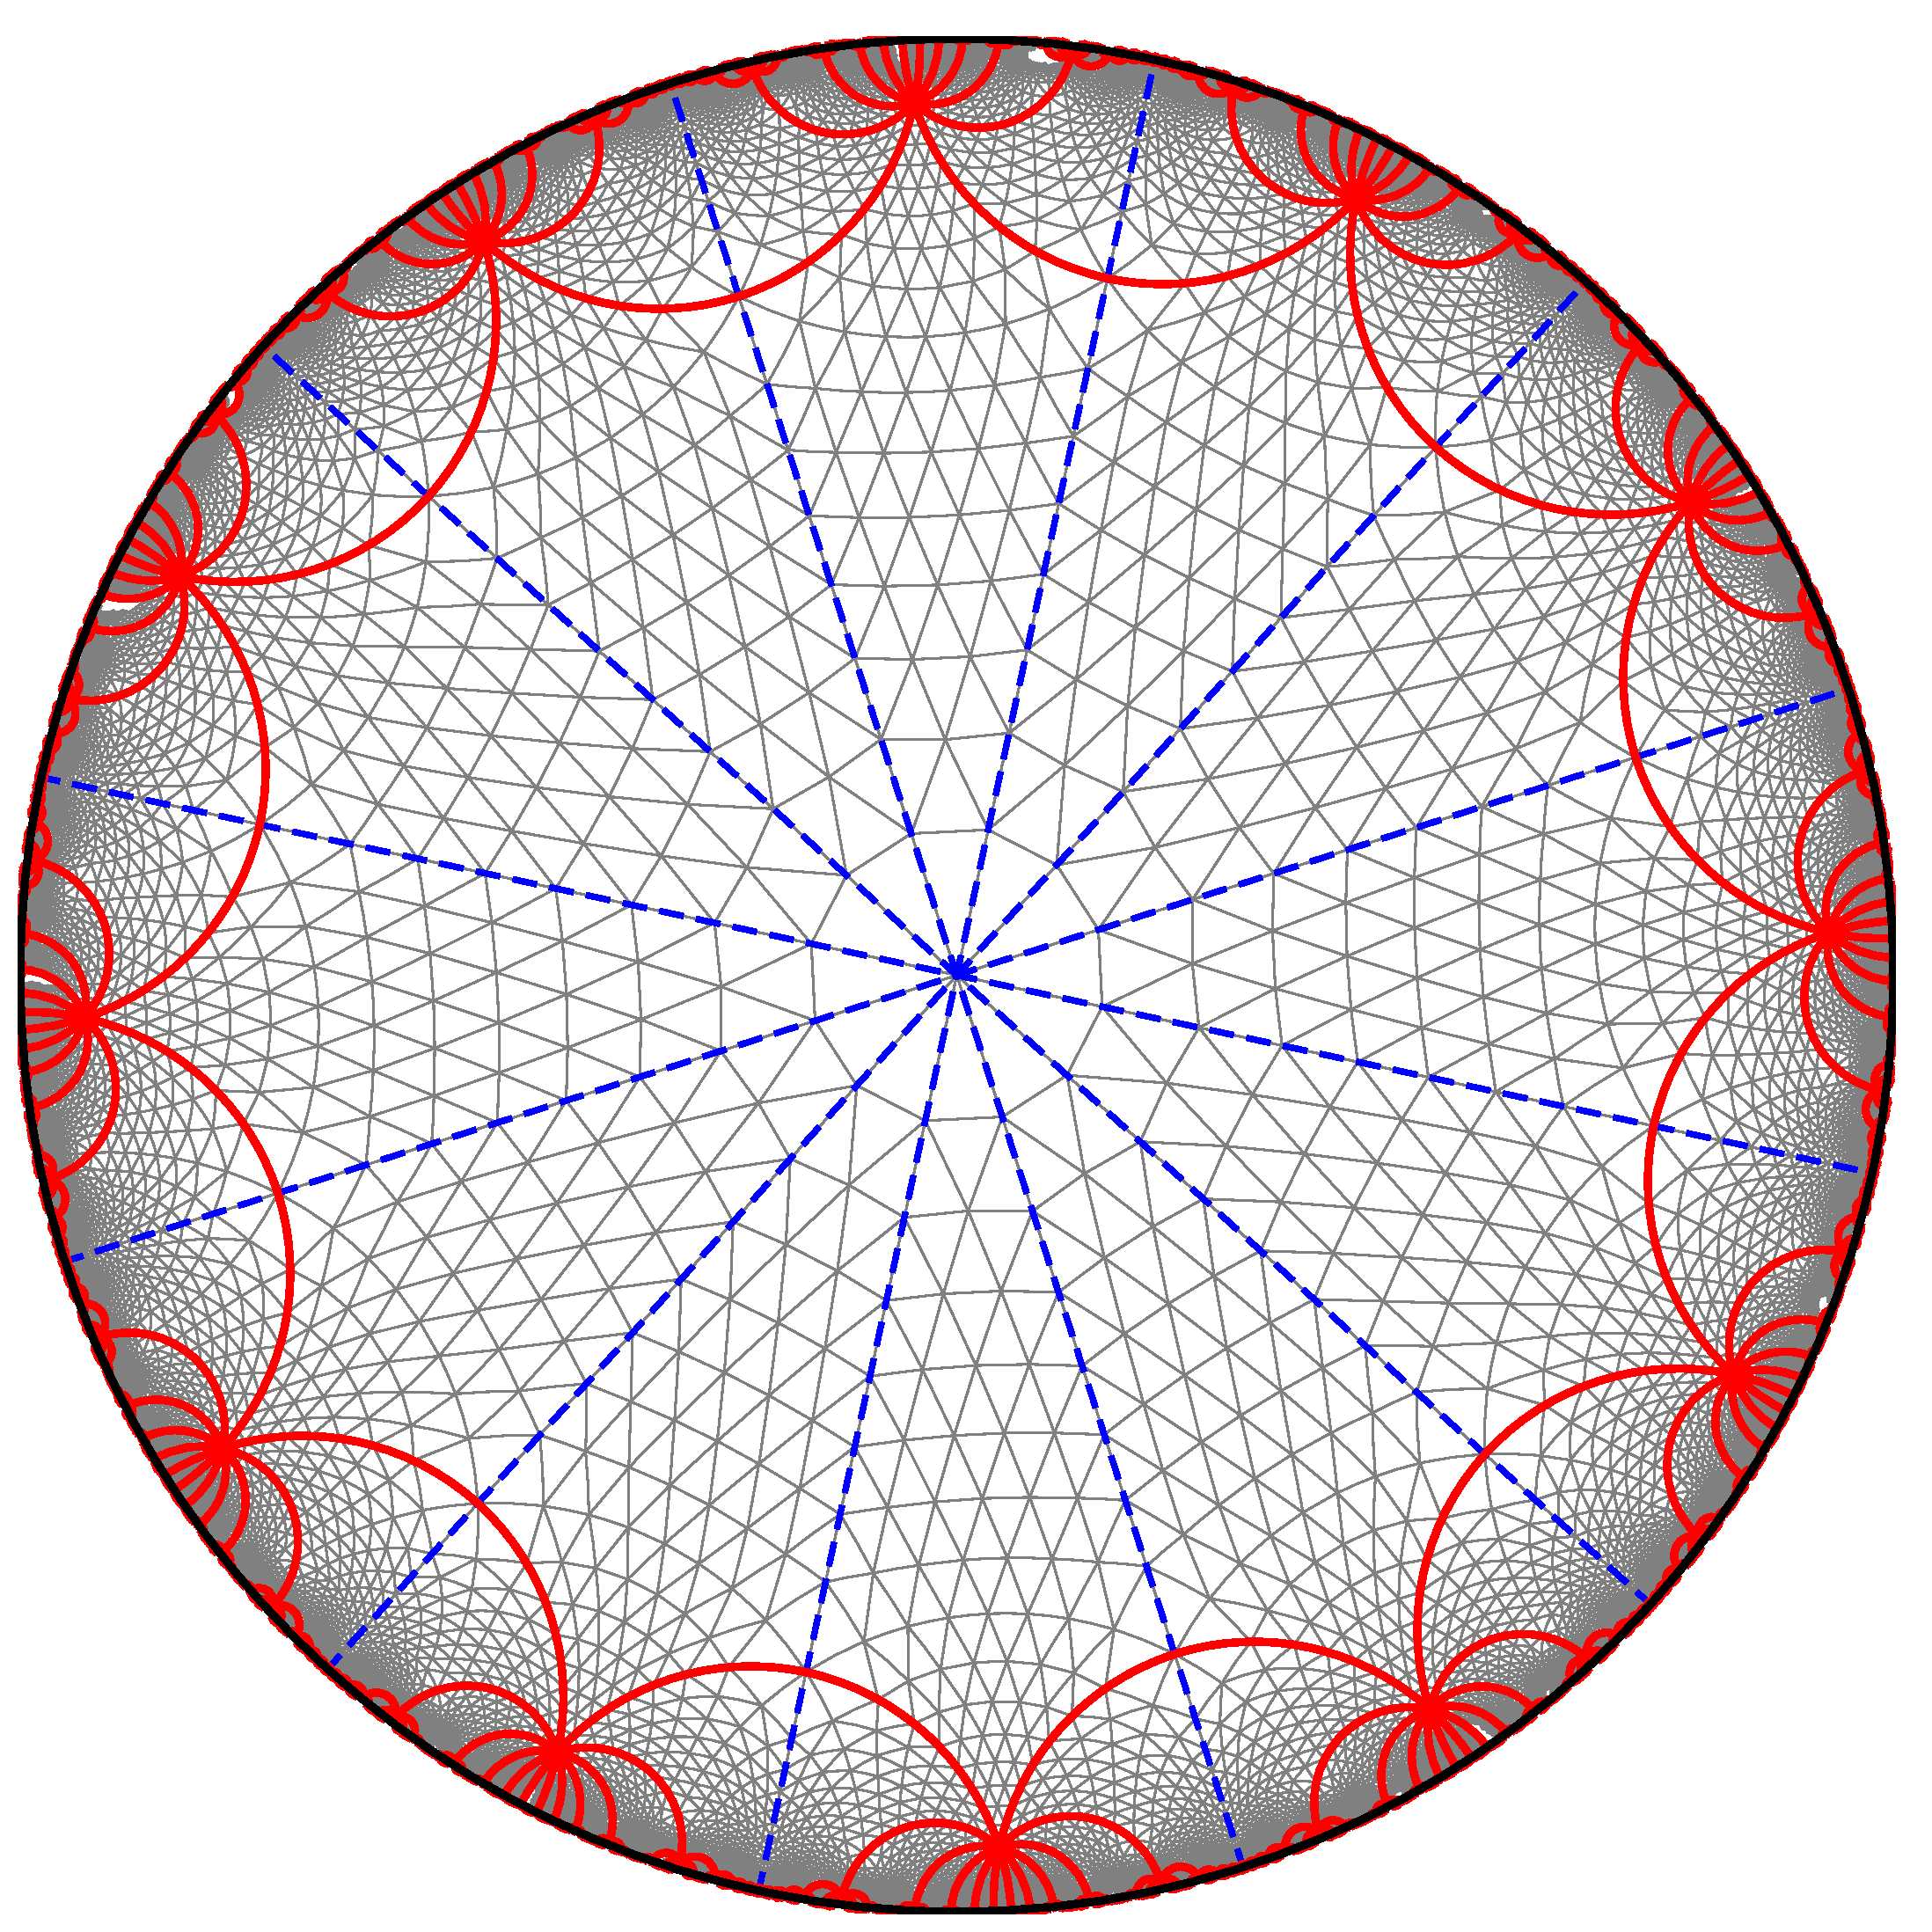
\includegraphics[width=0.48\linewidth]{cover04.png}
	\\
		Optimized PQ-Mesh with touching incircles
	\end{center}
\end{frame}

\begin{frame}
	\frametitle{More surfaces}
	\begin{center}
		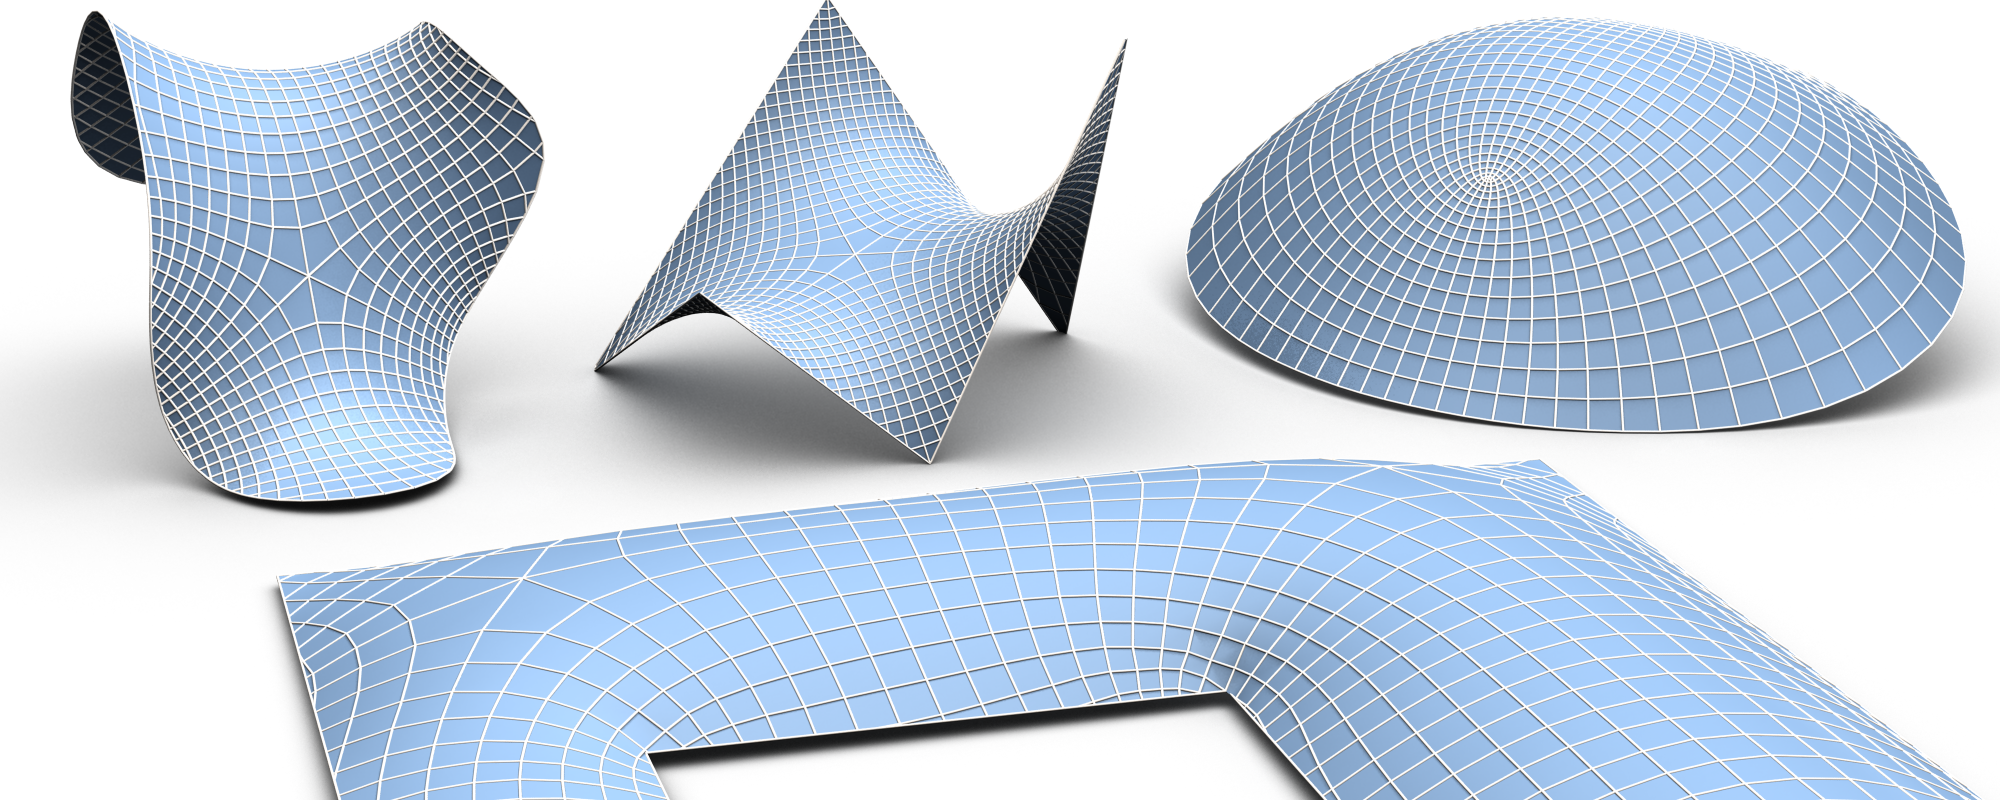
\includegraphics[width=\linewidth]{all_mesh.png}
	\end{center}
\end{frame}
\begin{frame}
	\frametitle{More surfaces}
	\begin{center}
		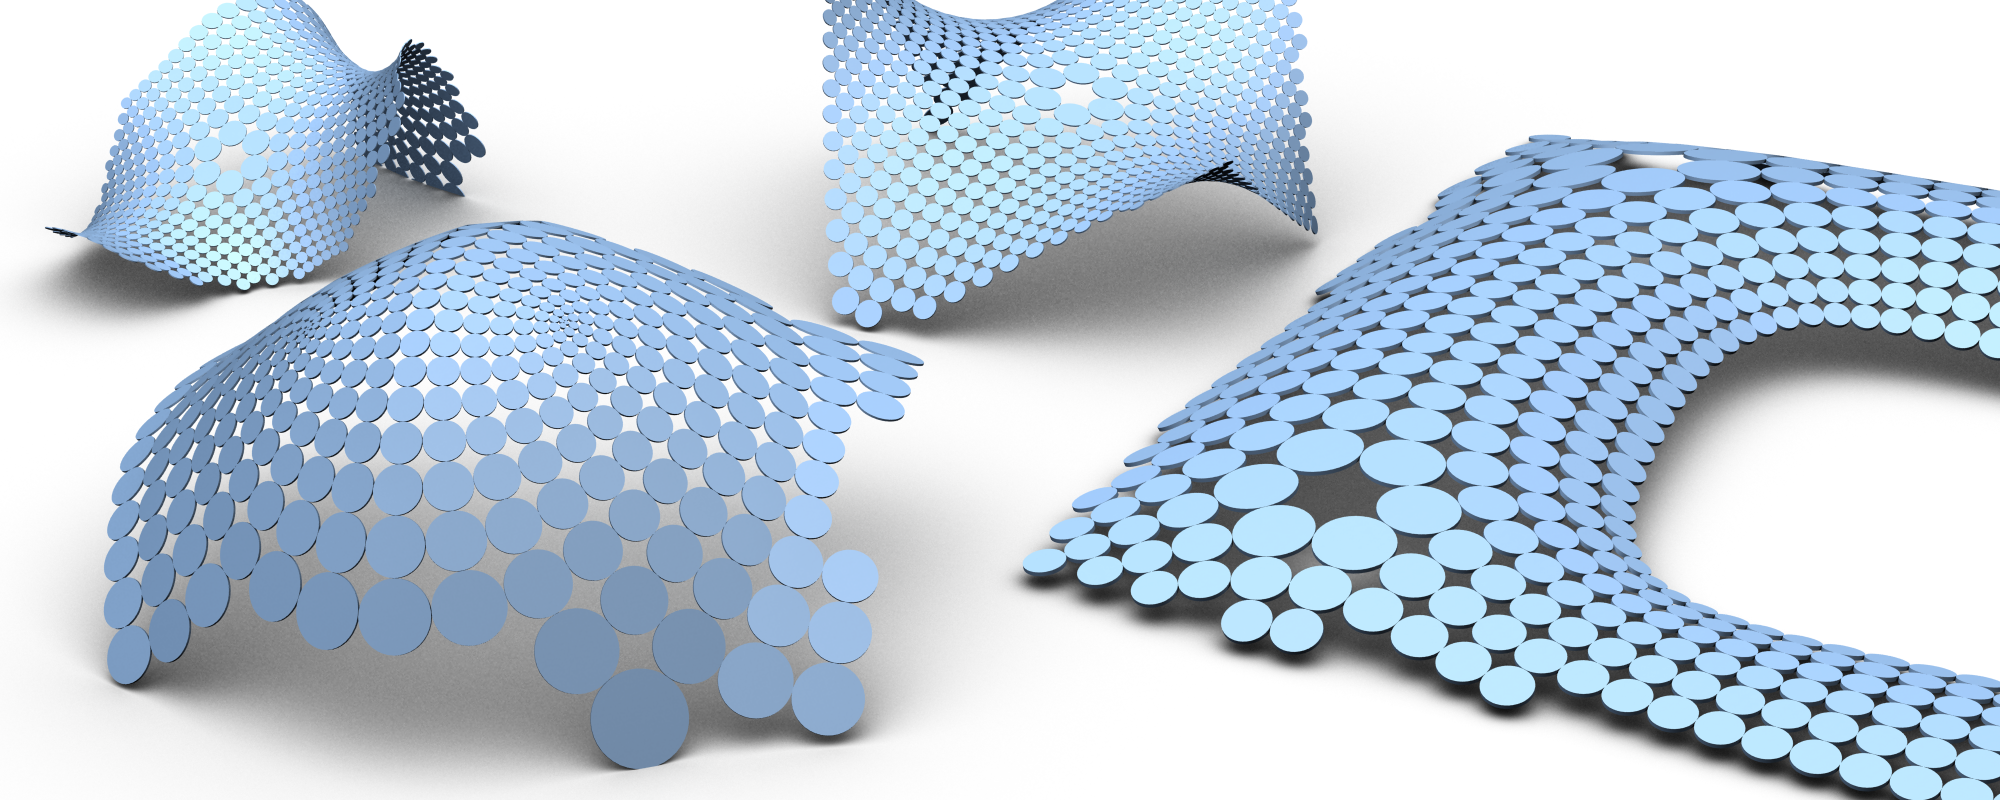
\includegraphics[width=\linewidth]{all_circles.png}\\
		\includegraphics[width=0.5\linewidth]{ellipsoid_disks01.png}
	\end{center}
\end{frame}

\begin{frame}
	\frametitle{Motivation}
	\begin{block}{From Discrete Differential Geometry}
        	Planar quadrilaterals with touching incircles approximate conformal curvature
		line (\emph{isothermically}) parameterized surfaces.
	\end{block}
	Was used before to create some minimal surfaces
	\begin{center}
	\includegraphics[width=0.3\linewidth]{cuboid01.png}
	\includegraphics[width=0.3\linewidth]{quad01.png}
	\includegraphics[width=0.3\linewidth]{Catenoid01.png}
	\end{center}
\end{frame}

\begin{frame}
	\frametitle{Isothermic Parameterization}
	\begin{center}
		\includegraphics[width=0.45\linewidth]{roof_curvature_lines2.png}
		\includegraphics[width=0.45\linewidth]{roof_conformal.png}\\
		Curvature Lines and Conformal $\rightarrow$ Isothermic.\\
		\includegraphics[width=0.6\linewidth]{roof_isothermic.png}
	\end{center}
\end{frame}


\begin{frame}
	\frametitle{Algorithm Outline}
	\begin{center}
		Isothermic Parameterization of a Triangle Mesh\\
		$\downarrow$\\
		Quad-Panel Generation\\
		$\downarrow$\\
		PQ/Incircle Optimization\\
		\vcenteredhbox{\includegraphics[width=0.28\linewidth]{cover02_no_vectors.png}}
		\vcenteredhbox{$\rightarrow$}
		\vcenteredhbox{\includegraphics[width=0.28\linewidth]{cover03_no_directions.png}}
		\vcenteredhbox{$\rightarrow$}
		\vcenteredhbox{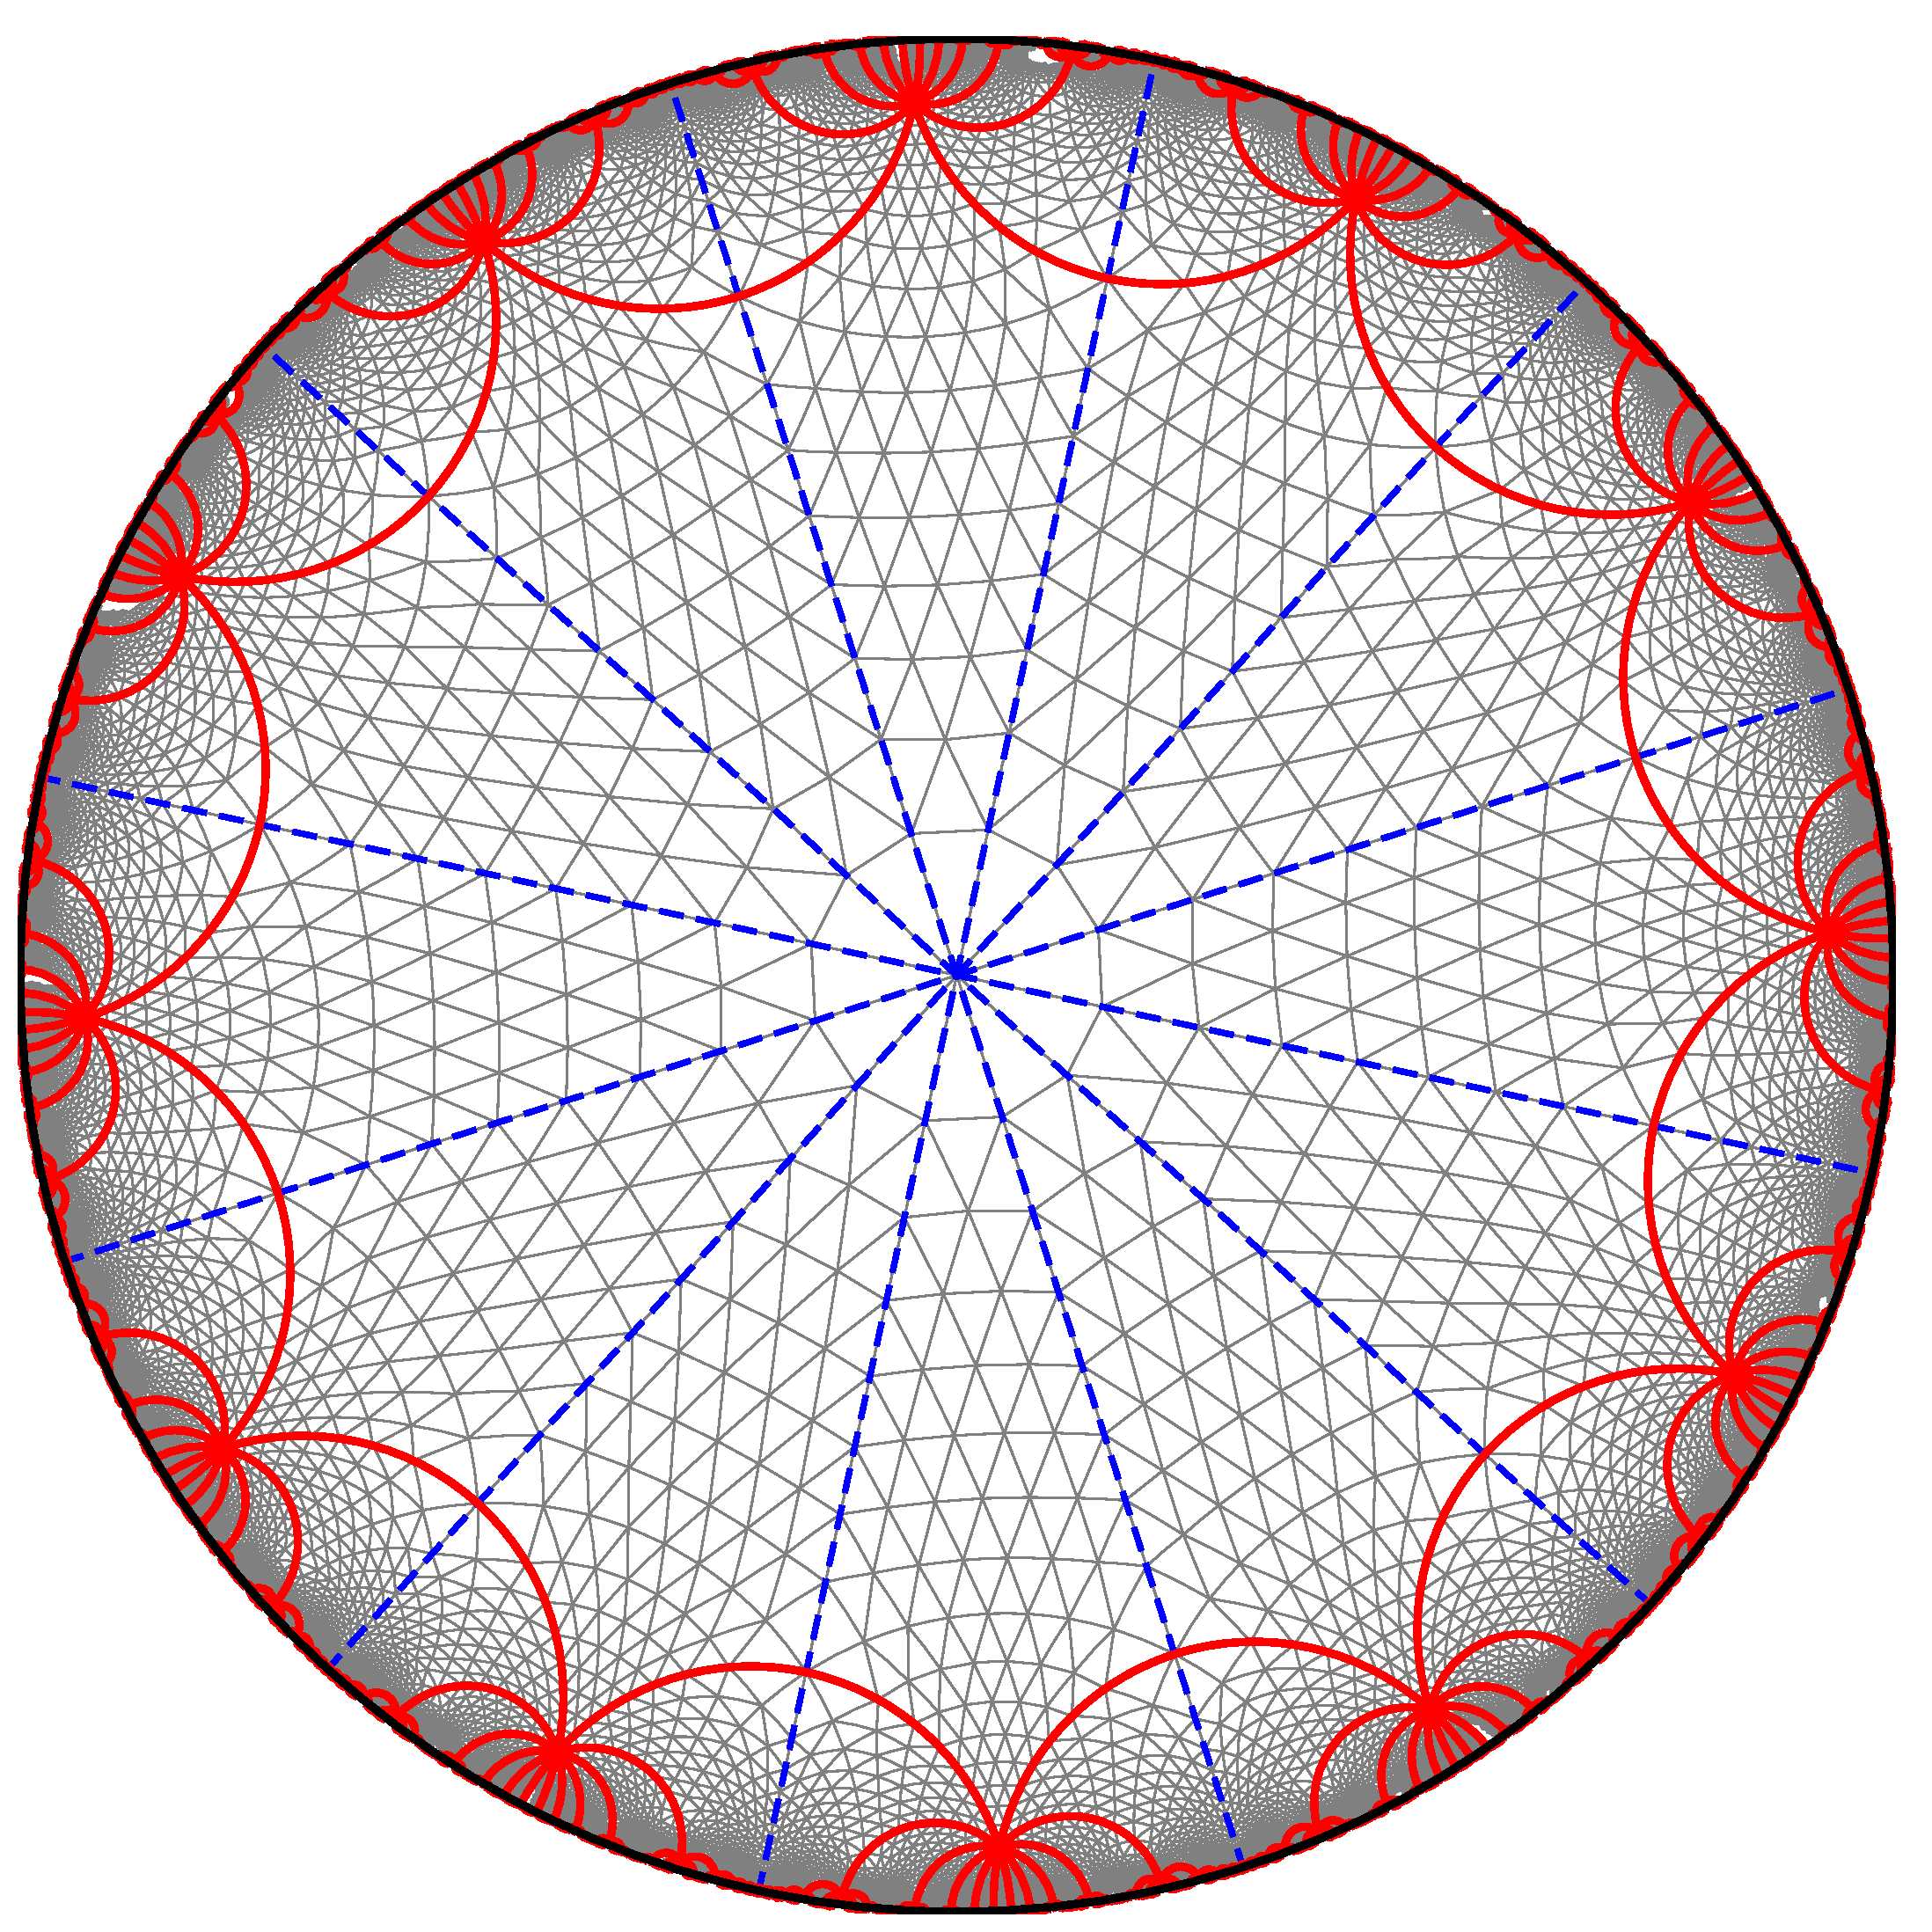
\includegraphics[width=0.28\linewidth]{cover04.png}}
	\end{center}
\end{frame}


\begin{frame}
  \frametitle{Discrete Conformal Parameterizations}
  	\begin{block}{Discrete Conformal Parameterization}
        	A map to the plane that mimmics the angle preserving property of smooth
		conformal maps.
	\end{block}
%  	\begin{block}{Degrees of Freedom}
%        	Boundary conditions and glocal scale are parameters
%	\end{block}
	\begin{center}
		\vcenteredhbox{\includegraphics[width=0.3\linewidth]{circle_domain.png}}
		\vcenteredhbox{$\rightarrow$}
		\vcenteredhbox{\includegraphics[width=0.3\linewidth]{circle.png}}\\
		Classical Riemann-Map to the Circle
	\end{center}
\end{frame}

\begin{frame}
  \frametitle{Discrete Conformal Parameterizations}
  Conformal maps with different boundary conditions.\\
	\includegraphics[width=0.25\linewidth]{conformal_isometric.png}
	\includegraphics[width=0.25\linewidth]{conformal_rectangle.png}
	\includegraphics[width=0.2\linewidth]{conformal_polygon.png}
	\includegraphics[width=0.25\linewidth]{conformal_curvature.png}\\
	\includegraphics[width=0.25\linewidth]{conformal_isometric_domain.png}
	\includegraphics[width=0.25\linewidth]{conformal_rectangle_domain.png}
	\includegraphics[width=0.2\linewidth]{conformal_polygon_domain.png}
	\includegraphics[width=0.25\linewidth]{conformal_curvature_domain.png}\\
\vspace{0.5cm}
\tiny{Algorithm: B. Springborn, P. Schr\"oder, U. Pinkall. Conformal Equivalence of Triangle Meshes. \\
ACM Transactions on Graphics 27:3 [Proceedings of ACM SIGGRAPH 2008]}
\end{frame}

\begin{frame}
	\frametitle{Curvature Boundary Conditions}
	\includegraphics[width=0.8\linewidth]{boundary_closeup.png}
\end{frame}

%\begin{frame}
%	\frametitle{Principle Curvature Directions}
%	\includegraphics[width=1.3\linewidth]{cover_directions.png}
%\end{frame}

\begin{frame}
  \frametitle{Curvature Boundary Conditions}
\scalebox{1.5} {
  \input{./image/boundary_condition.pdf_t}
}
Boundary angle sum $\theta$ at a boundary vertex
\end{frame}

\begin{frame}
  \frametitle{Curvature Boundary Conditions}
	\begin{center}
	\vcenteredhbox{\includegraphics[width=0.45\linewidth]{conformal_curvature_domain.png}}
	\vcenteredhbox{$\rightarrow$}
	\vcenteredhbox{\includegraphics[width=0.45\linewidth]{conformal_curvature.png}}\\
	Curvature boundary conditions and a singularity with angle 540$^\circ$
	\end{center}
\end{frame}


\begin{frame}
	\frametitle{Quasiisothermic Parameterization}
	\begin{block}{Quasiisothermic Parameterization}
        	We call a conformal parameterization with curvature boundary conditions
		a \emph{quasiisothermic parameterization}
	\end{block}
	\begin{center}
		\includegraphics[width=0.7\linewidth]{dach02_quality.png}
	\end{center}
\end{frame}

\begin{frame}
  \frametitle{Mesh Generation}
	\begin{center}
	\vcenteredhbox{\includegraphics[width=0.47\linewidth]{cover02_no_vectors.png}}
	\vcenteredhbox{$\rightarrow$}
	\vcenteredhbox{\includegraphics[width=0.47\linewidth]{cover03_no_directions.png}}\\
	Quad-Mesh Generation
	\end{center}
\end{frame}

\begin{frame}
	\frametitle{Optimization}
	\begin{block}{Variational Principle}
		Linear combination of energies
        	\begin{equation*}
		  E := 
		  \lambda_1 E_{\mathrm{planar}} + 
		  \lambda_2 E_{\mathrm{incircle}} + 
		  \lambda_3 E_{\mathrm{touch}}
		\end{equation*}
	\end{block}
\begin{itemize}
\item $E_{\mathrm{planar}}$ is some planarity term
\item $E_{\mathrm{incircle}}$ is due to 
	A.~Schiftner, M.~H\"obinger, J.~Wallner, and H.~Pottmann. 2009. \emph{Packing circles and spheres on surfaces.} ACM Trans. Graph. 28
\item $E_{\mathrm{touch}}$ critical for touching incircles
\end{itemize}
\end{frame}

\begin{frame}
  \frametitle{Touching Circles Energy}
	\begin{block}{Touching Circles Energy}
		\begin{equation*}
  E_{\mathrm{touch}}(\mathrm{\it{ij}})=
  \left(\cot\frac{\beta^j_l}{2}\cot\frac{\beta^i_r}{2} - 
\cot\frac{\beta^j_r}{2}\cot\frac{\beta^i_l}{2}\right)^2.
		\end{equation*}
	\end{block}
	\begin{center}
\input{../figures/e_touching_circles.pdf_t}
	\end{center}
\end{frame}


\begin{frame}
  \frametitle{Curvature Boundary Conditions}
	\begin{center}
	\vcenteredhbox{\includegraphics[width=0.47\linewidth]{incircles.png}}
	\vcenteredhbox{$\rightarrow$}
	\vcenteredhbox{\includegraphics[width=0.47\linewidth]{incircles_touch.png}}\\
	Optimization of the energy
	\end{center}
\end{frame}

\begin{frame}
  \frametitle{Optimization}
	\begin{center}
	\vcenteredhbox{\includegraphics[width=0.47\linewidth]{cover03_no_directions.png}}
	\vcenteredhbox{$\rightarrow$}
	\vcenteredhbox{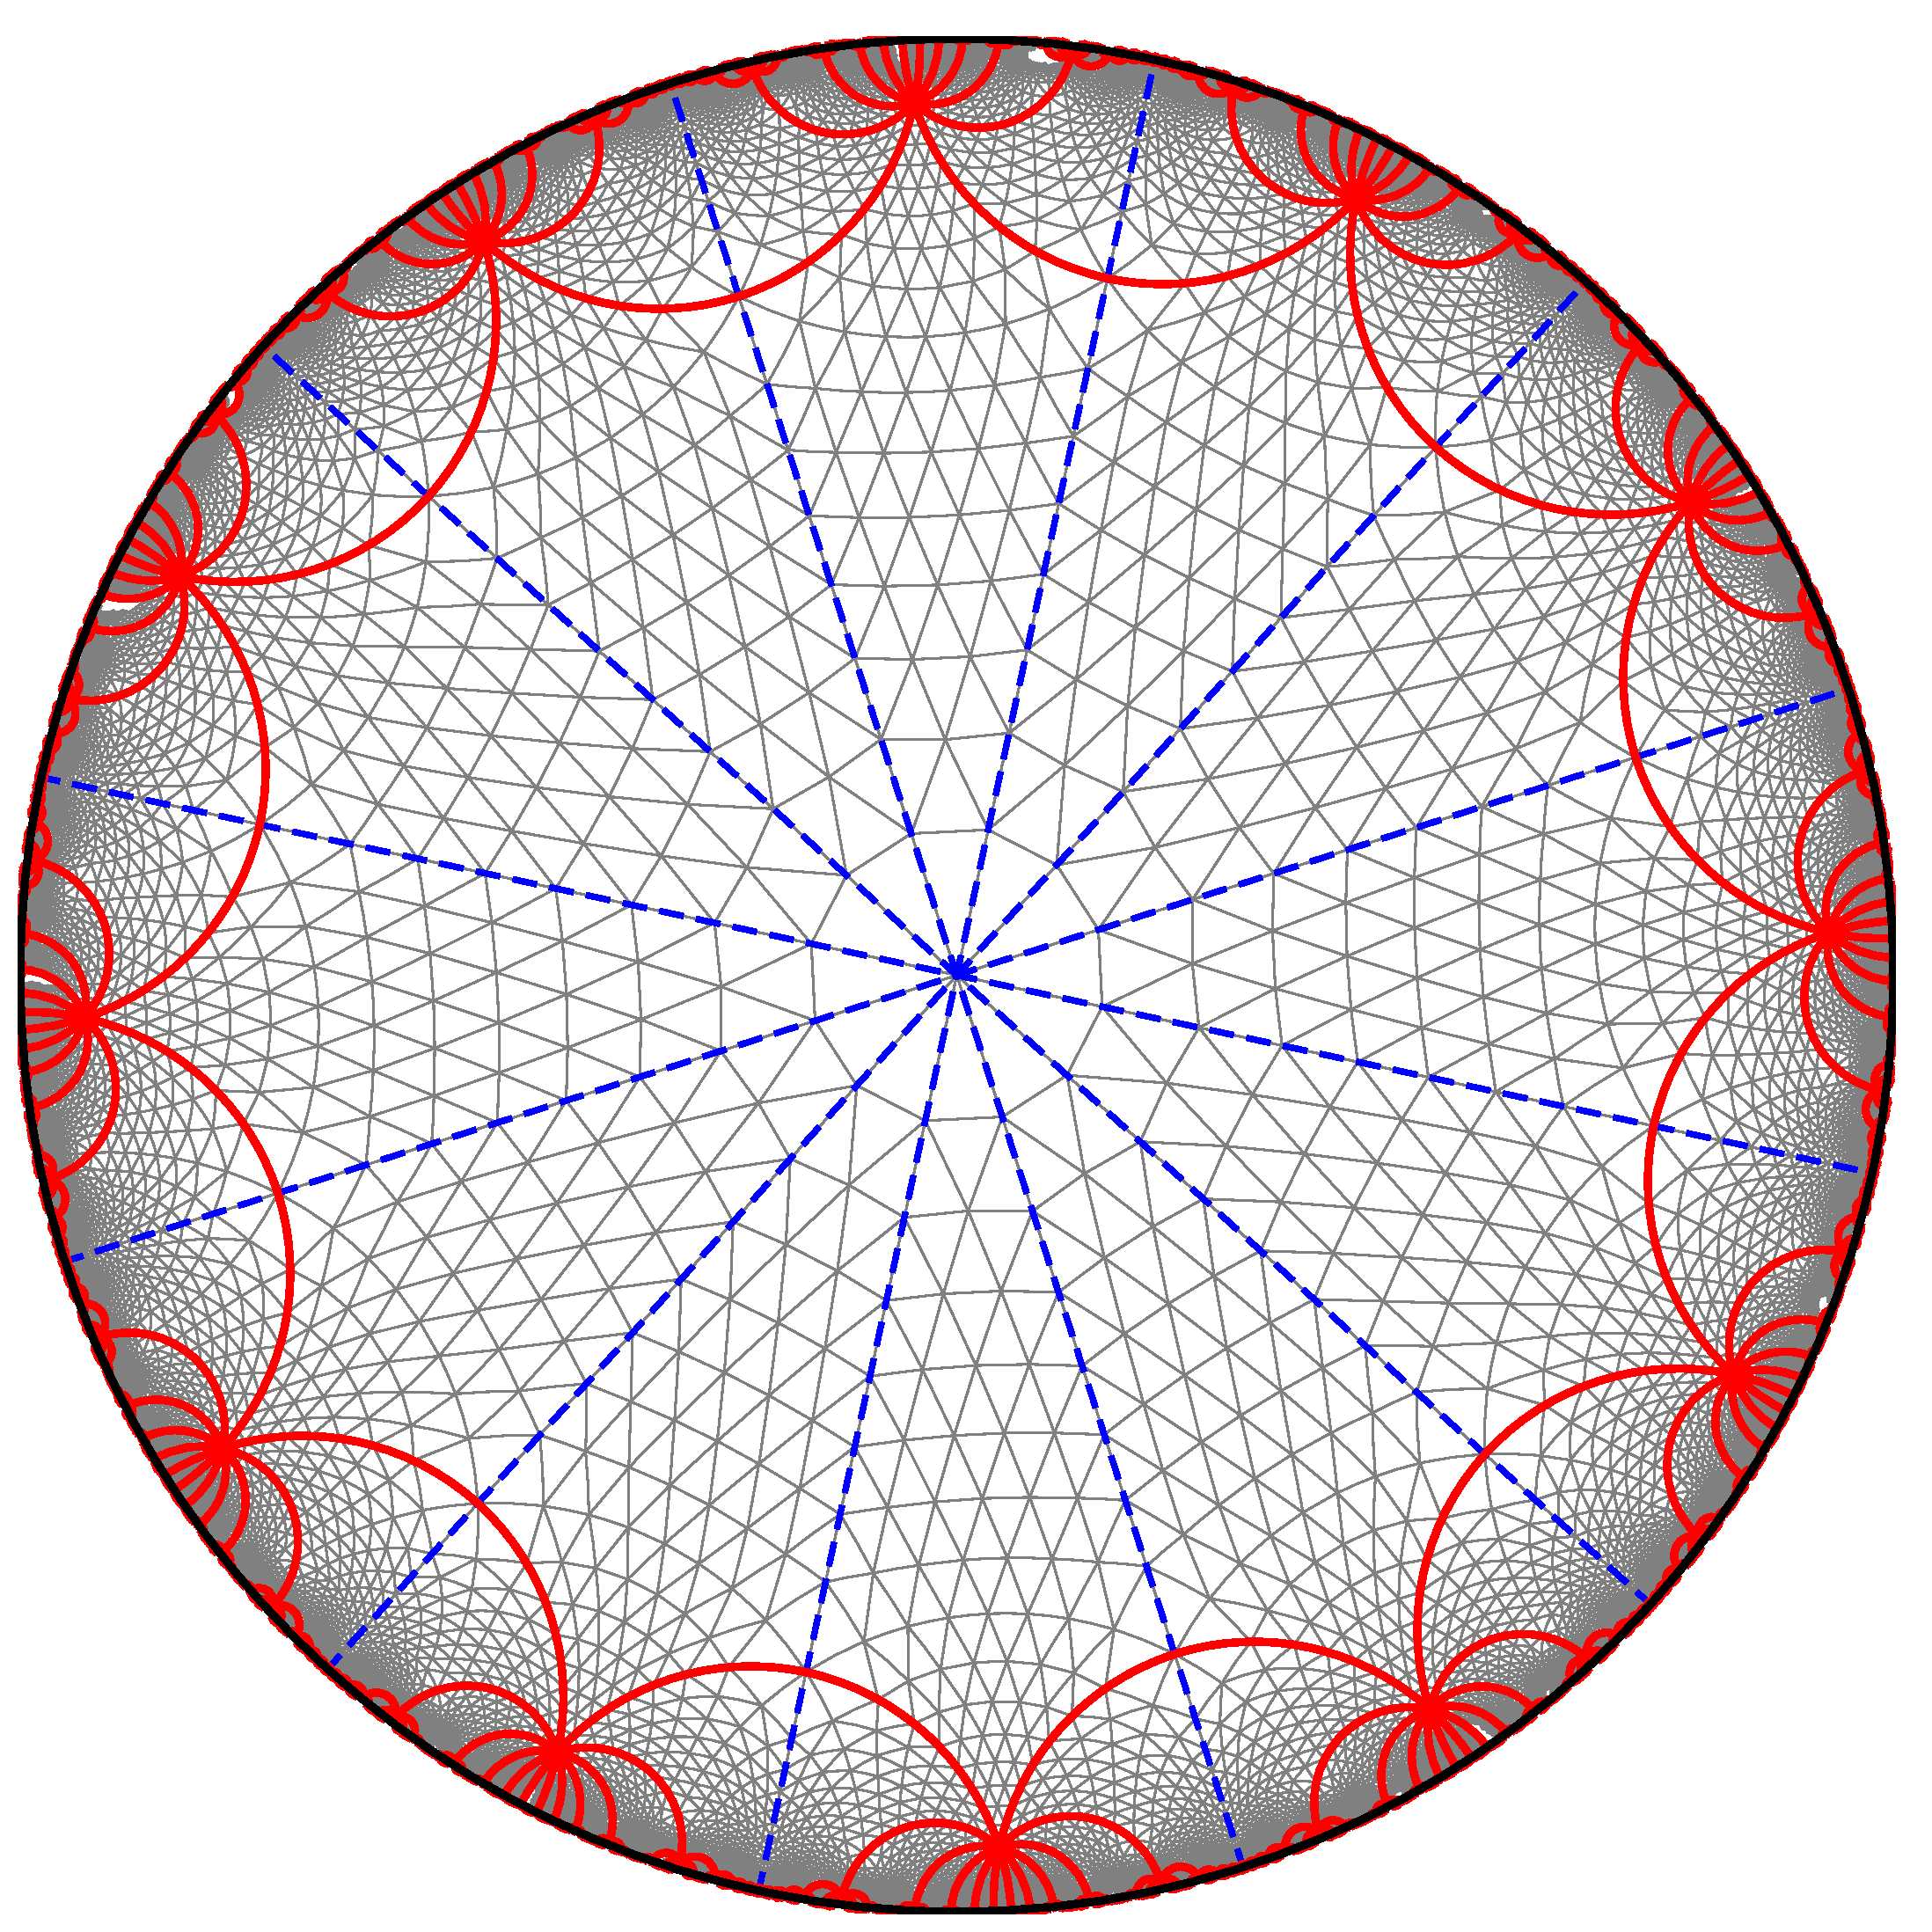
\includegraphics[width=0.47\linewidth]{cover04.png}}\\
	Optimization of big meshes needs a good guess $\rightarrow$ Quasiisothermic parameterizations
	\end{center}
\end{frame}

\begin{frame}
	\begin{center}
	\includegraphics[width=0.65\linewidth]{dach_example01_directions_thick.png}\\
	\includegraphics[width=0.65\linewidth]{dach_example01_circles.png}
	\end{center}
\end{frame}

\end{document}
